\documentclass[10pt, xcolor=table]{beamer}

\usepackage[utf8]{inputenc}
\usepackage{amsmath}
\usepackage{amsfonts}
\usepackage{amssymb}
\newcommand*\themecol{\usebeamercolor[fg]{structure}}

\setbeamertemplate{navigation symbols}{}
 \setbeamertemplate{footline}[frame number]

\newcommand{\overbar}[1]{\mkern 1.5mu\overline{\mkern-1.5mu#1\mkern-1.5mu}\mkern 1.5mu}

\usepackage{tikz}
\usetikzlibrary{shapes.geometric, arrows}
\tikzstyle{prob} = [rectangle, minimum width=3cm, text width = 4.5cm, minimum height=1cm, text centered, draw=black, fill= blue!20]
\tikzstyle{stat} = [rectangle, minimum width=3cm,  text width = 4.5cm, minimum height=1cm, text centered, draw=black, fill= red!20]
\tikzstyle{arrow} = [thick,->,>=stealth]


\setlength{\parindent}{0pt}
\setlength{\parskip}{6pt}


\title{STAT 111\\
{\small Recitation 7}}

\author{Mo Huang}
\institute{Email: mohuang@wharton.upenn.edu \\
\vspace{0.25cm}
Office Hours: Wednesdays 3:00 - 4:00 pm, JMHH F96\\
\vspace{0.25cm}
Slides: \url{github.com/mohuangx/STAT111-Spring2019} }


\date{March 22, 2019}


\begin{document}

\begin{frame}
\titlepage
\end{frame}

\begin{frame}{Estimation Summary}
\begin{itemize}\itemsep2ex
\vspace*{2ex}
\item Binomial parameter $\theta$:
\begin{itemize}
\item[] Estimate: $p$
\item[] 95\% confidence interval: $p \pm \sqrt{1/n}$
\end{itemize}
\item Mean $\mu$:
\begin{itemize}
\item[] Estimate: $\overbar{x}$
\item[] 95\% confidence interval: $\overbar{x} \pm 2\frac{s}{\sqrt{n}}$
\end{itemize}
\item Difference between proportions $\theta_1 - \theta_2$:
\begin{itemize}
\item[] Estimate: $p_1 - p_2$
\item[] 95\% confidence interval: ${p_1 - p_2 \pm  \sqrt{ \frac{1}{n} +  \frac{1}{m}}}$
\end{itemize}
\item Difference between means $\mu_1 - \mu_2$:
\begin{itemize}
\item[] Estimate: $\overbar{x}_1 - \overbar{x}_2$
\item[] 95\% confidence interval: $\overbar{x}_1 - \overbar{x}_2 \pm 2 \sqrt{\frac{s_1^2}{n} + \frac{s_2^2}{m}}$
\end{itemize}
\vspace*{1ex}
{\footnotesize \item[Note:] $$s = \sqrt{\frac{x_1^2  + x_2^2 + \cdots + x_n^2 - n(\overbar{x}^2)}{{ n-1}}}.$$}
\end{itemize}
\end{frame}

\begin{frame}{Linear Regression}
\begin{itemize}
\setlength{\itemsep}{8pt}
\item How does the growth height of a plant in a greenhouse depend on the amount of water that we give it?
\item Let $x$ be the amount of water we plan to give the plant (fixed).
\item Let $Y$ be the (future) growth height of a plant (random variable).
\item {\themecol Linear Regression Model}: for the $i$th observation,
\vspace{0.25cm}

\begin{itemize}
\setlength{\itemsep}{8pt}
\item Mean of $Y_i$ = $\alpha + \beta x_i$, $\qquad\qquad$ Variance of $Y_i$ = $\sigma^2$.
\end{itemize}
\end{itemize}
\begin{figure}
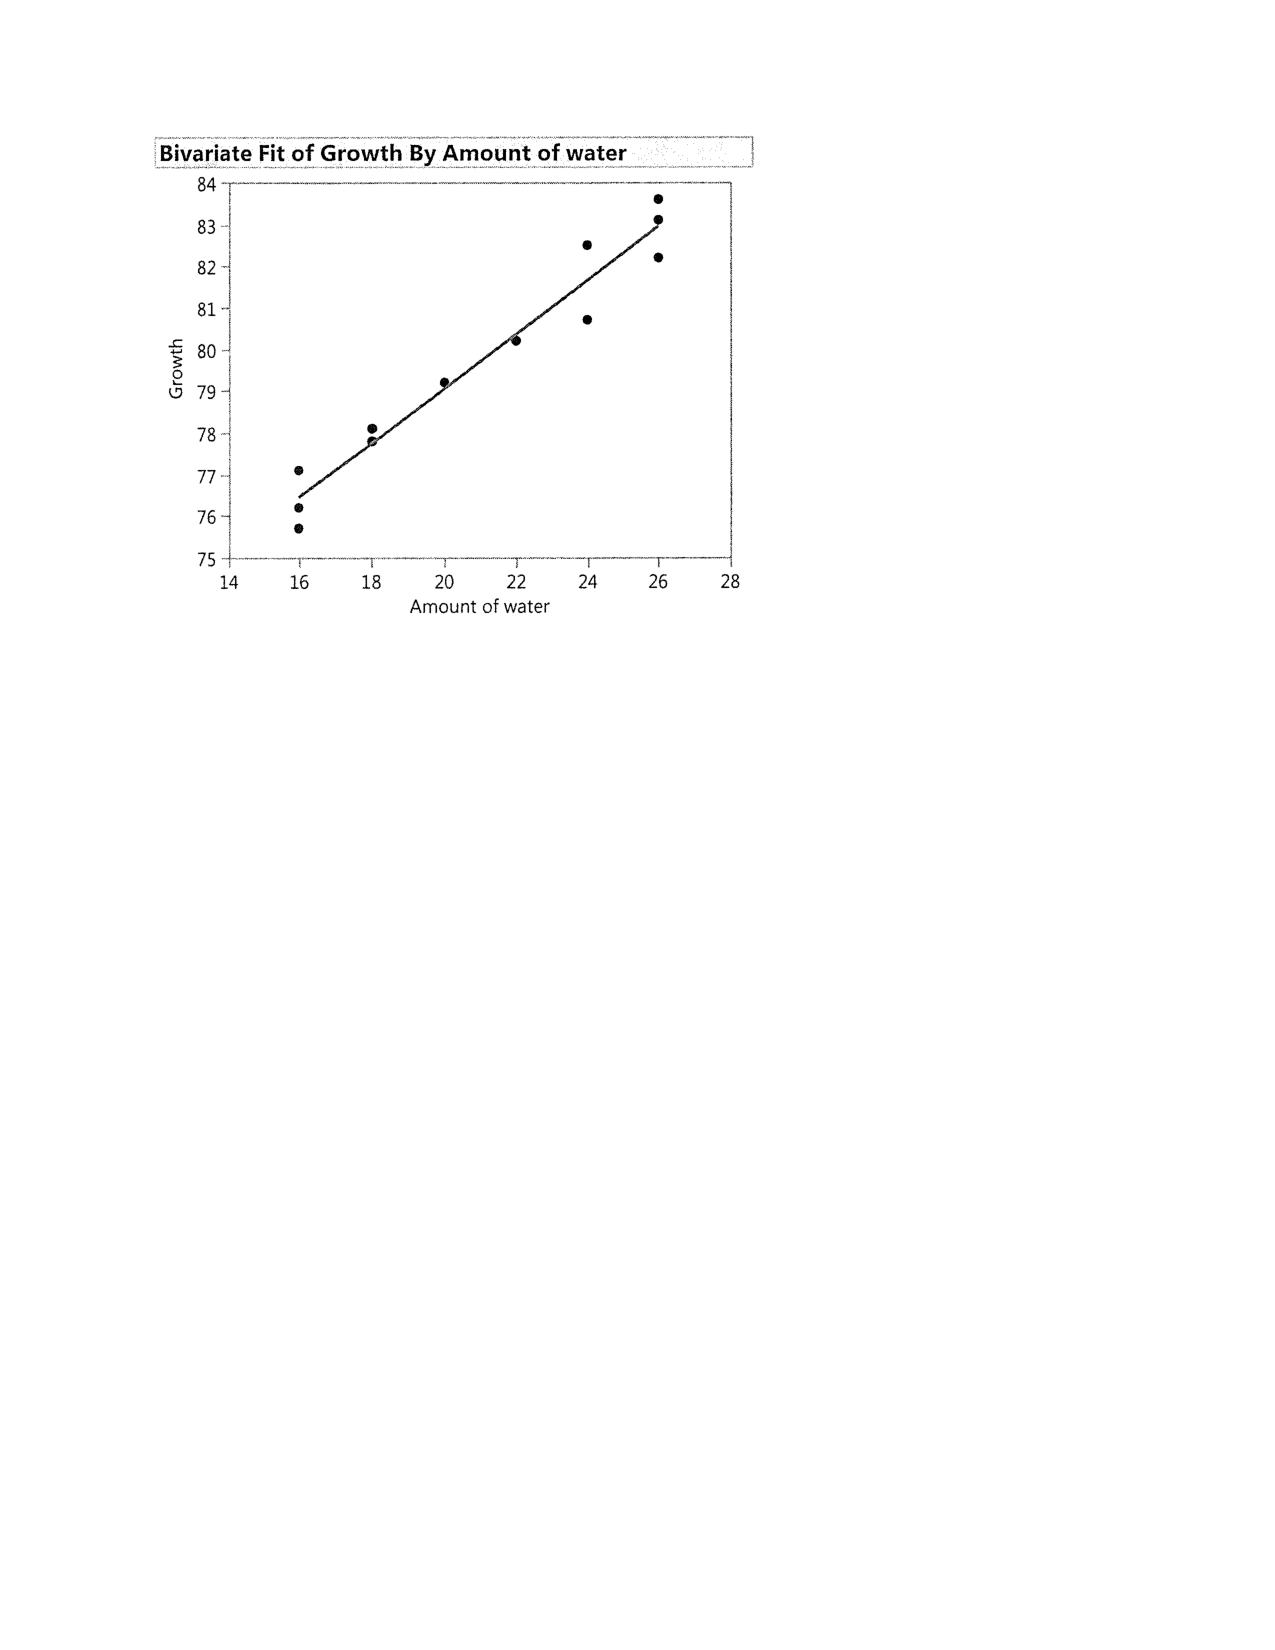
\includegraphics[width = 0.4\textwidth]{images/rec9_1}
\caption{Data: $(x_1, y_1), (x_2, y_2), \dots, (x_n, y_n)$}
\end{figure}
\end{frame}

\begin{frame}{Linear Regression}
\small
\begin{itemize}
\setlength{\itemsep}{6pt}
\item Mean of $Y_i$ = $\alpha + \beta x_i$, Variance of $Y_i$ = $\sigma^2$. How do we estimate $\alpha$, $\beta$?
\end{itemize}
\begin{align*}
\text{Calculate:} \quad s_{xx} &= x_1^2 + x_2^2 + \cdots + x_n^2 - n(\overline{x}^2) = \sum_{i=1}^n x_i^2 - n(\overline{x}^2)\\
s_{yy} &= y_1^2 + y_2^2 + \cdots + y_n^2 - n(\overline{y}^2) = \sum_{i=1}^n y_i^2 - n(\overline{y}^2) \\
s_{xy} &= x_1y_1 + x_2y_2 + \cdots + x_ny_n - n(\overline{x}\overline{y}) = \sum_{i=1}^n x_i y_i - n(\overline{x}\overline{y}).
\end{align*}
\vspace{-0.25cm}
\begin{itemize}
\setlength{\itemsep}{8pt}
\item Estimate $\beta$ by $b$ and $\alpha$ by $a$:
{\themecol \begin{align*}
 b &= s_{xy}/s_{xx}\\
a &= \overline{y} - b\overline{x}
\end{align*}}
\vspace{-0.5cm}
\item Estimate $\sigma^2$ by $s_r^2$:
$${\themecol s_r^2 = (s_{yy} - b^2 s_{xx})/(n-2).}$$
\item How accurate is the estimate $b$ of $\beta$?
$$\text{Standard deviation of }b:{ \themecol \frac{s_r}{\sqrt{s_{xx}}}} \quad \Rightarrow \quad 95\% \text{ C.I. }{\themecol b \pm 2\frac{s_r}{\sqrt{s_{xx}}}}$$
\end{itemize}
\end{frame}

\begin{frame}{Example}
\begin{figure}
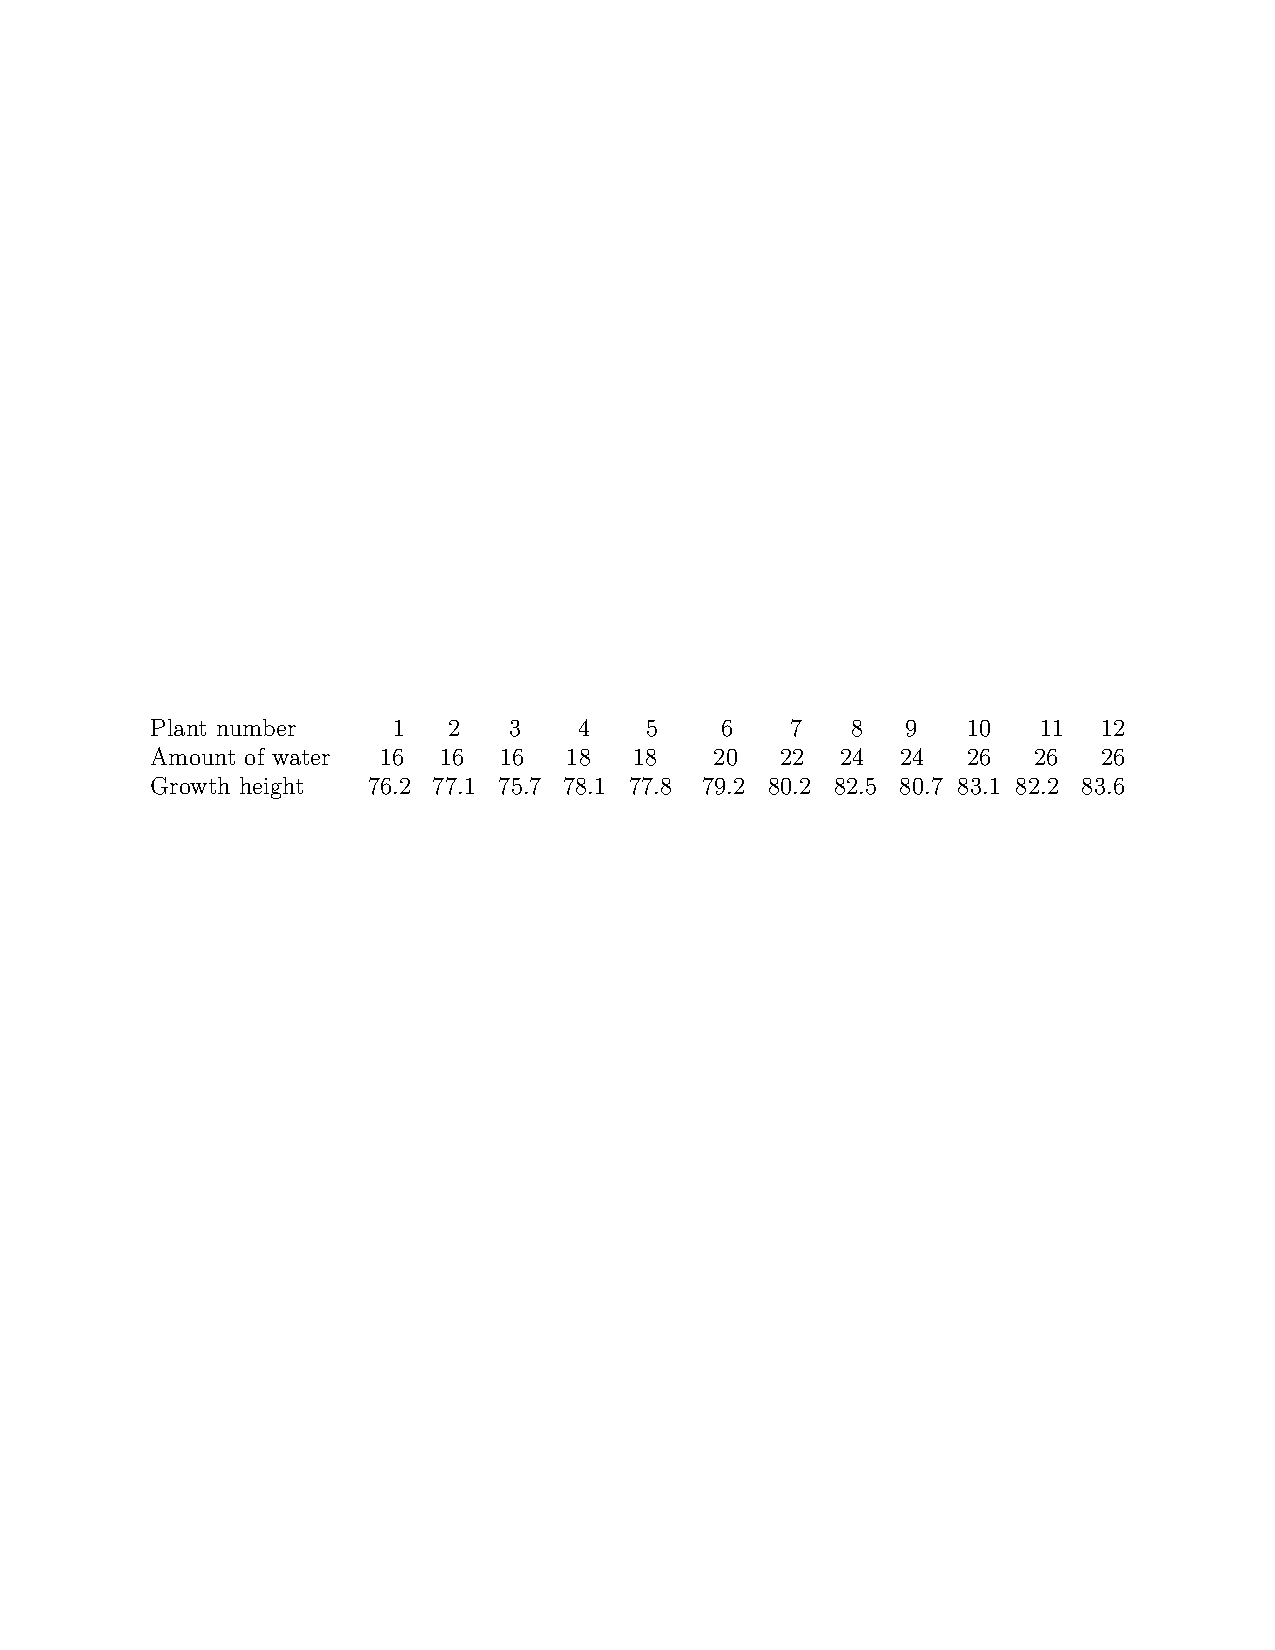
\includegraphics[width = 0.95\textwidth]{images/rec9_2}
\end{figure}
\begin{itemize}
\setlength{\itemsep}{10pt}
\item $\overline{x} = 21, \overline{y} =  79.7, s_{xx} = 188, s_{yy} = 83.54, s_{xy} = 122.4$
\item<2-> Estimate $\alpha,\ \beta$
\uncover<3->{\color{red}
\begin{align*}
b &= s_{xy}/s_{xx} = 0.6511 \\[6pt]
a &= \overline{y} - \beta\overline{x} = 79.7 - (0.6511)(21) = 66.03
\end{align*}}
\vspace*{-4ex}
\item<3-> Estimate $\sigma^2$
\uncover<4->{\color{red}
\[s_r^2 = \frac{83.54 - (0.6511)^2(188)}{10} = 0.3850\]
}
\vspace*{-3ex}
\item<4-> Find a 95\% C.I. for $\beta$.
\uncover<5->{\color{red}
\[
95\% \text{ C.I. for } b : 0.6511 \pm 2\frac{\sqrt{0.3850}}{\sqrt{188}} \Rightarrow (0.56, 0.74)
\]
}

\end{itemize}

\end{frame}


\end{document}


